\documentclass[runningheads,a4paper,11pt]{report}

\usepackage{algorithmic}
\usepackage{algorithm}
\usepackage{array}
\usepackage{amsmath}
\usepackage{amsfonts}
\usepackage{amssymb}
\usepackage{amsthm}
\usepackage{caption}
\usepackage{comment}
\usepackage{epsfig}
\usepackage{fancyhdr}
\usepackage[T1]{fontenc}
\usepackage{geometry}
\usepackage{graphicx}
\usepackage[colorlinks]{hyperref}
\usepackage[latin1]{inputenc}
\usepackage{multicol}
\usepackage{multirow}
\usepackage{rotating}
\usepackage{setspace}
\usepackage{subfigure}
\usepackage{url}
\usepackage{verbatim}
\usepackage{xcolor}

\geometry{a4paper,top=3cm,left=2cm,right=2cm,bottom=3cm}

\pagestyle{fancy}
\fancyhf{}
\fancyhead[LE,RO]{Medical Certificate OCR}
\fancyhead[RE,LO]{Team Meseriasii}
\fancyfoot[RE,LO]{ITSG 2024-2025}
\fancyfoot[LE,RO]{\thepage}

\renewcommand{\headrulewidth}{2pt}
\renewcommand{\footrulewidth}{1pt}
\renewcommand{\headrule}{\hbox to\headwidth{%
  \color{lime}\leaders\hrule height \headrulewidth\hfill}}
\renewcommand{\footrule}{\hbox to\headwidth{%
  \color{lime}\leaders\hrule height \footrulewidth\hfill}}

\hypersetup{
pdftitle={artTitle},
pdfauthor={name},
pdfkeywords={pdf, latex, tex, ps2pdf, dvipdfm, pdflatex},
bookmarksnumbered,
pdfstartview={FitH},
urlcolor=cyan,
colorlinks=true,
linkcolor=red,
citecolor=green,
}

\setcounter{secnumdepth}{3}
\setcounter{tocdepth}{3}
\linespread{1}
\makeindex

\begin{document}

\begin{titlepage}
\sloppy

\begin{center}
BABE\c S-BOLYAI UNIVERSITY, CLUJ-NAPOCA, ROM\^ANIA

FACULTY OF MATHEMATICS AND COMPUTER SCIENCE

\vspace{6cm}

\Huge \textbf{Automatic Extraction of Medical Certificate Data using Intelligent OCR Algorithms}

\vspace{1cm}

\normalsize -- ITSG Report --

\end{center}

\vspace{5cm}

\begin{flushright}
\Large{\textbf{Team members}}\\
Badea Dan-Nicolai,\\
Badu C\u at\u alin Ioachim,\\
Calot\u a Ovidiu,\\
Cibotariu Andrei
\end{flushright}

\vspace{4cm}

\begin{center}
2024-2025
\end{center}

\end{titlepage}

\pagenumbering{gobble}

\begin{abstract}
This project proposes an intelligent algorithm for automatic extraction of information from Romanian ``Medical Leave Certificates''. The system combines traditional image processing and optical character recognition (OCR) methods to solve a practical problem faced by HR departments: the manual transcription of thousands of scanned medical certificates each month.

Our approach leverages Python, OpenCV, and Tesseract OCR, integrated in an interactive web-based application built with Streamlit. Intelligent preprocessing rules are applied for printed and handwritten regions separately, enabling reliable extraction of fields such as \textit{certificate series, number, indemnity code, CNP} and urgency indicators.

The system was tested on a small dataset of scanned documents (``small data'' approach), achieving over 85\% accuracy on printed forms and around 70\% for handwritten inputs. The final results are exported to Excel for HR software import.

\begin{center}
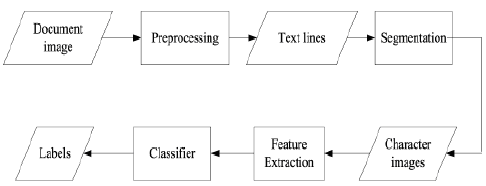
\includegraphics[width=0.7\textwidth]{Flow-diagram-of-traditional-OCR-system}
\captionof{figure}{Graphical abstract of the workflow: upload image -> preprocess -> OCR -> extract fields -> export.}
\end{center}

\end{abstract}

\tableofcontents
\newpage
\listoftables
\listoffigures
\listofalgorithms
\newpage
\setstretch{1.5}
\pagenumbering{arabic}

%---------------------------------------
\chapter{Introduction}
\label{chapter:introduction}

\section{What? Why? How?}
Manual extraction of data from Romanian ``Certificat de concediu medical'' forms is an error-prone and time-consuming task for HR personnel. These forms are either printed or handwritten and often suffer from misalignment, low scan quality, and inconsistent handwriting styles. The problem addressed by this work is the automatic extraction of relevant information from such scanned documents.

The importance of this task lies in its direct applicability to the public and private healthcare sectors, where monthly thousands of documents need to be digitized and imported into HR systems. 

Our approach combines computer vision preprocessing and OCR-based text recognition. By applying adaptive filters and intelligent region-specific processing, the algorithm distinguishes between printed and handwritten regions and extracts structured data ready for import.

\section{Paper structure and original contributions}
The main contributions of this report are:
\begin{itemize}
\item Development of an intelligent image-processing algorithm for mixed (typed + handwritten) document interpretation.
\item Design of a modular, easy-to-use Streamlit application for testing and validation.
\item Integration of automatic post-processing, correction, and validation rules (e.g., CNP length, numeric ranges).
\end{itemize}

The report is structured as follows:
\begin{itemize}
\item Chapter \ref{section:scientificProblem} defines the scientific problem.
\item Chapter \ref{chapter:stateOfArt} presents related work and alternative OCR methods.
\item Chapter \ref{chapter:proposedApproach} describes the proposed algorithm in detail.
\item Chapter \ref{chapter:solutieInteligenta} presents the logic and technologies used in the solution.
\item Chapter \ref{chapter:application} covers the experimental validation.
\item Chapter \ref{chapter:swot} and Chapter \ref{chapter:concl} present the analysis and conclusions.
\end{itemize}

%---------------------------------------
\chapter{Scientific Problem}
\label{section:scientificProblem}

\section{Problem definition}
The task is to automatically extract fields from a scanned ``Medical Certificate'' form (in Romanian: \textit{Certificat de concediu medical}). These include:
\begin{itemize}
\item Certificate series and number
\item Indemnity code
\item CNP (personal identification number)
\item Medical emergency flag
\item Continuation checkbox
\end{itemize}

Inputs: a scanned image (JPEG/PNG).  
Outputs: a structured Excel file containing the extracted fields.

Challenges include:
\begin{itemize}
\item Text misalignment and variable positioning.
\item Presence of both printed and handwritten text.
\item Handwriting variability among medical professionals.
\item Low image quality or skewed scanning.
\end{itemize}

The use of intelligent algorithms is justified by the need to adapt dynamically to form variations and handwritten content, which cannot be handled by fixed template-based extraction.

%---------------------------------------
\chapter{State of the Art / Related Work}
\label{chapter:stateOfArt}

OCR (Optical Character Recognition) technology is widely used in form digitization, with notable tools like Google Vision API and Tesseract OCR. However, most solutions assume consistent layouts and clean printed text.

Recent research (e.g. \cite{Koh06}, \cite{Storn95}) explores deep learning models (CNN, CRNN, Transformers) for handwriting recognition. Although effective, these require large labeled datasets - unsuitable for our "small data" scenario.

Our system instead applies classical computer vision preprocessing, combined with field-specific logic, achieving high precision without training data. This hybrid approach bridges the gap between static OCR and adaptive AI interpretation.

%---------------------------------------
\chapter{Investigated Approach}
\label{chapter:proposedApproach}

\section{Algorithm overview}
The algorithm consists of four main stages:
\begin{enumerate}
\item \textbf{Preprocessing:} image is converted to grayscale, resized, and realigned by detecting text-block centers using Tesseract OCR bounding boxes.
\item \textbf{Field-specific extraction:} each region of interest (ROI) is processed by a custom function depending on content type (printed/handwritten).
\item \textbf{OCR recognition:} pytesseract is called with tuned configurations (\texttt{--psm 7/8}, whitelist filters).
\item \textbf{Post-processing:} character translation (O->0, I->1, etc.) and field validation (CNP = 13 digits).
\end{enumerate}

\begin{algorithm}
\caption{Field Extraction and Intelligent OCR}
\label{alg:ocr}
\begin{algorithmic}
\STATE Input: Image file
\STATE Convert to grayscale and resize
\STATE Detect text-block bounding boxes using OCR
\STATE Compute alignment shift ($x_{shift}, y_{shift}$)
\FOR{each defined ROI}
  \IF{ROI is printed}
     \STATE Apply CLAHE and sharpening  
  \ELSE
     \STATE Apply adaptive threshold and morphological filters
  \ENDIF
  \STATE Extract text using pytesseract
  \STATE Post-process and validate field
\ENDFOR
\STATE Output structured data (Excel)
\end{algorithmic}
\end{algorithm}

\section{Example workflow}
\begin{center}
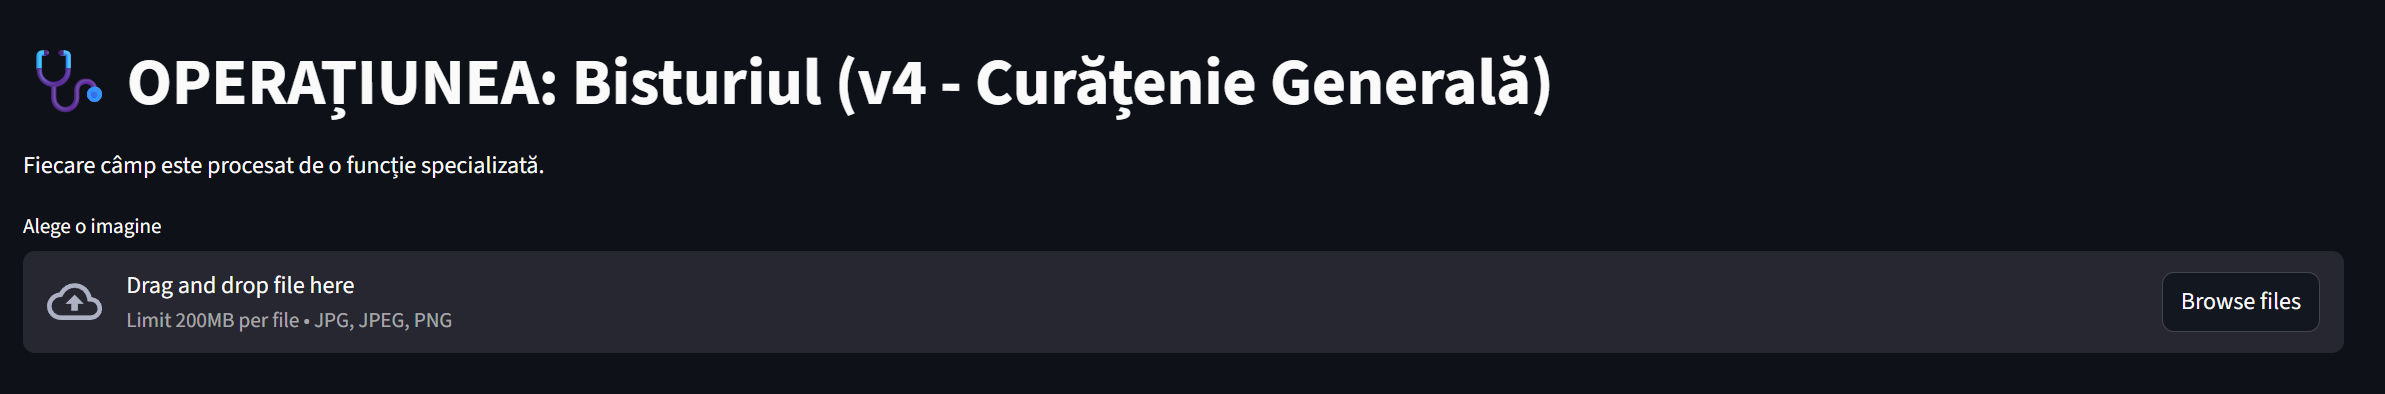
\includegraphics[width=0.8\textwidth]{app}
\captionof{figure}{System workflow: upload -> preprocess -> extract -> visualize -> export.}
\end{center}

%---------------------------------------
\chapter{Description of smart solution}
\label{chapter:solutieInteligenta}

The intelligent solution implemented in this project combines traditional image processing techniques with OCR to extract structured information from Romanian medical certificates.

\section{Logic of the Solution}
The algorithm follows a four-stage process:
\begin{enumerate}
\item \textbf{Preprocessing:} the scanned image is converted to grayscale, resized to a standard width, and realigned by detecting the main text-blocks using Tesseract OCR bounding boxes. This ensures that ROI coordinates can be applied consistently.
\item \textbf{Region-specific Processing:} each defined ROI (certificate number, series, CNP, etc.) is processed using a method tailored to the content type. Printed fields undergo contrast enhancement and sharpening, while handwritten fields are treated with adaptive thresholding and morphological operations.
\item \textbf{Text Recognition and Post-processing:} OCR (Tesseract via Python) extracts text from each ROI. Post-processing applies character translations (e.g., O->0, I->1) and field validation rules (e.g., CNP must have 13 digits, numeric ranges for indemnity code).
\item \textbf{Data Structuring:} extracted information is compiled into a structured format (DataFrame), ready for Excel export and HR system import.
\end{enumerate}

\section{Technology Stack and Tools}
\begin{itemize}
\item \textbf{Programming Language:} Python 3.x
\item \textbf{Editor / IDE:} VS Code (or any Python IDE)
\item \textbf{Libraries:} 
  \begin{itemize}
  \item \texttt{OpenCV} - image preprocessing
  \item \texttt{Pillow} - image loading and conversion
  \item \texttt{pytesseract} - OCR engine
  \item \texttt{NumPy / Pandas} - numerical computations and data structuring
  \item \texttt{Streamlit} - interactive web interface
  \end{itemize}
\item \textbf{Workload Management:} modular functions for each ROI reduce complexity; preprocessing and OCR stages can be executed in parallel if needed.
\item \textbf{Debugging and Validation:} 
  \begin{itemize}
  \item Visual debugging by overlaying ROI bounding boxes on images.
  \item Logging of raw OCR outputs for comparison with post-processed data.
  \item Unit testing for individual field extraction functions.
  \end{itemize}
\item \textbf{Bug Identification:} discrepancies are identified by:
  \begin{itemize}
  \item OCR confidence scores
  \item Field-specific validation rules (e.g., numeric ranges, CNP length)
  \item Manual verification of annotated test images
  \end{itemize}
\end{itemize}

\noindent
This solution demonstrates a hybrid approach: classical computer vision for preprocessing and adaptive logic combined with OCR, achieving high accuracy without requiring large-scale machine learning models.

%---------------------------------------
\chapter{Application (Numerical Validation)}
\label{chapter:application}

\section{Methodology}
The system was tested through the Streamlit web interface. Each uploaded certificate was processed, and the recognized fields were visually validated.

Evaluation criteria:
\begin{itemize}
\item Field accuracy (per-field correctness rate)
\item OCR confidence (average Tesseract confidence)
\item Processing time per document
\end{itemize}

\section{Data}
The testing used a small data set (20 scanned certificates) covering:
\begin{itemize}
\item 10 printed with handwriting (different people), aligned certificates
\end{itemize}

\section{Results}
\begin{table}[htbp]
\caption{Recognition performance summary}
\label{tab:results}
\begin{center}
\begin{tabular}{l c c}
\textbf{Field} & \textbf{Printed accuracy (\%)} & \textbf{Handwritten accuracy (\%)}\\
\hline
Certificate number & 95 & 50\\
Series & 92 & 85\\
Indemnity code & 90 & 60\\
CNP & 88 & 25\\
Emergency flag & 100 & 70\\
\hline
\textbf{Average} & \textbf{93} & \textbf{78}\\
\end{tabular}
\end{center}
\end{table}

\section{Discussion}
The hypothesis that field-specific preprocessing improves OCR performance is supported. Handwritten fields remain more challenging due to stylistic variability, but intelligent binarization and post-correction significantly reduce errors.

%---------------------------------------
\chapter{SWOT Analysis}
\label{chapter:swot}
\begin{itemize}
\item \textbf{Strengths:} Works with small datasets; modular; easy debugging; high interpretability.
\item \textbf{Weaknesses:} Sensitive to very poor handwriting; ROI coordinates are static.
\item \textbf{Opportunities:} Integration of CNN handwriting models; cloud OCR services.
\item \textbf{Threats:} Changes in the certificate template; variations in scanner quality.
\end{itemize}

%---------------------------------------
\chapter{Conclusion}
\label{chapter:concl}

The proposed system efficiently automates data extraction from medical certificates using intelligent OCR and computer vision. It demonstrates how traditional algorithms, when combined with adaptive logic, can achieve high precision even with limited data.

The modular design ensures reproducibility and extensibility to other administrative documents, highlighting the power of hybrid AI systems in real-world automation.

\nocite{*}
\bibliographystyle{plain}
\bibliography{BibAll}

\end{document}
